\section{CNN Classifier}

\subsection{Region of Interest Size}

We generate locations for the potential merges from the skeletons using the algorithm in Section 3.2.
From these locations we extract a cubic region of interest.
We experimented with three different region of interest side lengths: $800 \textrm{nm}$, $1200 \textrm{nm}$, and $1600 \textrm{nm}$. 
Side lengths of $1600 \textrm{nm}$ performed better on the training and validation data on our networks. 

\subsection{CNN Parameters}

We experimented with several different network architectures before deciding on the one presented in our paper. 
We considered two optimizers: stochastic gradient descent with Nesterov momentum and Adam~\cite{kingma2014adam}.
In addition we tried two different loss functions: binary cross entropy and mean squared error.
We also experimented with four different input sizes that correspond to different cube sizes output from the final max pooling layer. 
After running a brute force search over all of these possible architectures, we found that the best architecture used a SGD optimizer with Nesterov momentum, a mean squared error loss function, and an input size of $76 \times 76 \times 24$. 

\subsection{Architecture}

\begin{figure*}
	\centering
	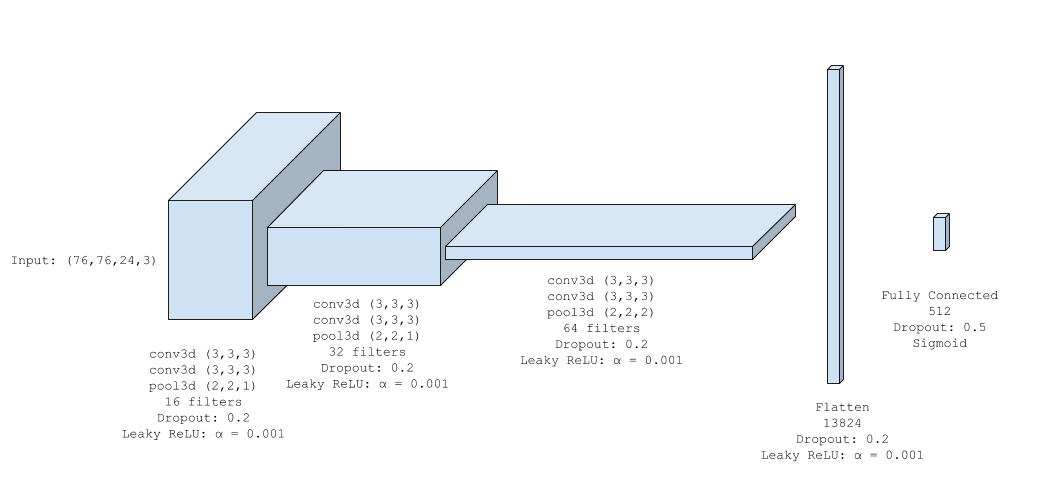
\includegraphics[width=0.9\linewidth]{./figures/architecture.png}
	\caption{The final architecture presented in this paper.}
	\label{fig:architecture}
\end{figure*}

Figure \ref{fig:architecture} shows the final architecture that produced the best results on the validation data. 
The input data was $76 \times 76 \times 24$ voxels with $3$ channels per voxel. 
This corresponds to an output size from the third max pooling layer of $6 \times 6 \times 6$. 
This flattens to a $13,824$-element vector and two dense layers of output size $512$ and $1$ follow. 
All activation layers are Leaky ReLU with $\alpha=0.001$ except for the final layer which has a sigmoid activation.